\documentclass{article}\usepackage[]{graphicx}\usepackage[]{color}
%% maxwidth is the original width if it is less than linewidth
%% otherwise use linewidth (to make sure the graphics do not exceed the margin)
\makeatletter
\def\maxwidth{ %
  \ifdim\Gin@nat@width>\linewidth
    \linewidth
  \else
    \Gin@nat@width
  \fi
}
\makeatother

\usepackage{Sweavel}


\usepackage{geometry}
 \geometry{
 a4paper,
 total={210mm,297mm},
 left=25mm,
 right=25mm,
 top=30mm,
 bottom=20mm,
 }
\begin{document}

\lstset{breaklines=true} % break long lines



\section*{\LARGE\centering\textcolor{blue}{Are there more python or javascript repositories on GitHub?}}

\subsection*{\Large\centering\textcolor{red}{Sruthi Singireddy \newline{April 20, 2015}}}

\subsection*{\Large\textcolor{black}{Overview}}

\subsection*{\Large\textcolor{black}{GitHub}}
\large{GitHub is an online hosting service for Git repository. GitHub was launched in April 2008 by Tom Preston-Werner, Chris Wanstrath and PJ Hyett. GitHub is mostly used for code and provides social networking functions like feeds, followers, wikis, social network graph that displays how developers work on their forks and which fork is newest. GitHub operates pastebin called Gist which is used for hosting code snippets and Speaker Deck which is a slide hosting service.}

GitHub offers distributed revision control and source code management. GitHub has Graphical User Interface (GUI), desktop and mobile integration unlike Git which is purely command line. GitHub has some exceptional features like access control and some collaboration tools like task management, wikis, bug tracking and feature request for every project. As of 2015, GitHub has 21.1 million repositories which makes numero one hosting service in the world.                             {\newline\textbf{[Source: http://en.wikipedia.org/wiki/GitHub]}

\subsection*{\Large\textcolor{black}{JavaScript}}
JavaScript, a dynamic programming language was originally named as LiveScript but was changed to JavaScript in September 1995. The language was developed by Brendan Eich in Netscape Communication Corporation.  JavaScript is a part of  web browsers which allow client-side script to interact with users, communicate asynchronously, change the document’s content. JavaScript is a prototype-based scripting language and is multi paradigm language as it supports object-oriented, imperative and functional programming paradigms.  JavaScript hugely differs from Java and they have very different semantics. {\newline\textbf{[Source:http://en.wikipedia.org/wiki/JavaScript]}}   

\subsection*{\Large\textcolor{black}{Python}}
   Python, a general purpose language was written by Van Rossum in 1996. Python is multi paradigm language as it supports object-oriented, structured programming paradigms, aspect oriented programming and functional programming. Python uses dynamic typing and it uses reference counting and cyclic detecting garbage collector for memory management. A significant feature of Python is late binding as it binds method and variable during execution. Python is a highly readable language. {\newline\textbf{[Source:http://en.wikipedia.org/wiki/Python]}}                                                                                             

\subsection*{\Large\textcolor{blue}{O\textcolor{black}{btaining the data}}}
The code chunk below obtains data from GitHub API and storing into csv files.
{\newline{\textbf{API} stands for Application Programming Interface. API is a set of standards and instructions for using web tools. It is software to software interface which means software applications communicate with each other. Software companies release their APIs to let developers design products based on the services.{\newline\textbf{[Source:http://money.howstuffworks.com/business-communications/how-to-leverage-an-api-for-conferencing1.htm]}}
\newline{In code chunk below I'm obtaining information of JavaScript and Python repositories from github API in JSON format. After obtaining data it is wriiten into respective CSV files}}}

\begin{Schunk}
\begin{Sinput}
library(jsonlite)
library(httr)
library(RCurl)

# get data in JSON format from GitHub
javascript <- fromJSON("https://api.github.com/search/repositories?q=language:javascript")
python <- fromJSON("https://api.github.com/search/repositories?q=language:python")

# javascript data is sent into CSV file
tmp <- lapply(javascript, function(u) lapply(u, function(x) if (is.null(x)) NA else x))
tmp <- lapply(tmp, as.data.frame)
tmp <- do.call(rbind, tmp)
write.csv(tmp, file = "javascripts.csv")

# python data is sent into CSV files
tmppython <- lapply(python, function(u) lapply(u, function(x) if (is.null(x)) NA else x))
tmppython <- lapply(tmppython, as.data.frame)
tmppython <- do.call(rbind, tmppython)
write.csv(tmppython, file = "python.csv")
\end{Sinput}
\end{Schunk}
\subsection*{\Large\textcolor{blue}{E\textcolor{black}{xploring and }\textcolor{blue}{ S}\textcolor{black}{ crubing the data}}}
After obtaining the data from the API, I'm capturing total repositories in both python and javascript.

\begin{Schunk}
\begin{Sinput}
# Comparision of the number of GitHub repositories of Python and JavaScript

library(jsonlite)
\end{Sinput}
\begin{Soutput}

Attaching package: 'jsonlite'

The following object is masked from 'package:utils':

    View
\end{Soutput}
\begin{Sinput}
library(plyr)
library(ggplot2)
library(scales)

url <- "https://api.github.com/"  # the GitHub API
path <- "search/repositories"  # Repositories path
searchjs <- "?q=language:javascript&sort=stars&order=desc"  # query string fetch javascript repos 
searchpython <- "?q=language:python&sort=stars&order=desc"  # query string fetch python repos 
\end{Sinput}
\end{Schunk}

\begin{Schunk}
\begin{Sinput}
# Paste0 allows us to concatenate all of the above into one long URL here is
# javascript version
URLjs <- paste0(url, path, searchjs)

# Here is the python version
URLpython <- paste0(url, path, searchpython)


# The above URL will create a page in json format We can read the json and
# convert it to a list using the jsonlite package
js = jsonlite::fromJSON(URLjs)

# Displaying the summary of the js variable
summary(js)
\end{Sinput}
\begin{Soutput}
                   Length Class      Mode   
total_count         1     -none-     numeric
incomplete_results  1     -none-     logical
items              68     data.frame list   
\end{Soutput}
\begin{Sinput}
# We can get the number of R Repositories simply by capturing the total
# count
repos.js <- js$total_count

# We can read the json and convert it to a list using the jsonlite package
py = jsonlite::fromJSON(URLpython)

# Displaying the summary of the py variable
summary(py)
\end{Sinput}
\begin{Soutput}
                   Length Class      Mode   
total_count         1     -none-     numeric
incomplete_results  1     -none-     logical
items              68     data.frame list   
\end{Soutput}
\begin{Sinput}
# We can get the number of python Repositories simply by capturing the total
# count
repos.python <- py$total_count
\end{Sinput}
\end{Schunk}
\subsection*{\Large\textcolor{black}{Results (\textcolor{blue}{M}\textcolor{black}{ore Exploring)}}}
The results show that javascript has 1291089 repositories and javascript has 633101 repositoriesin GitHub. These figures clearly show that \textbf{JavaScript has more repositories than Python in GitHub}

\begin{Schunk}
\begin{Sinput}
# Number of repositories in javascript
repos.js
\end{Sinput}
\begin{Soutput}
[1] 1291830
\end{Soutput}
\begin{Sinput}
# Number of repositories in python
repos.python
\end{Sinput}
\begin{Soutput}
[1] 633497
\end{Soutput}
\end{Schunk}

\subsection*{\Large\textcolor{black}{graphiNg}}
For the graphical presentation bar chart and line graph are drawn to show the clear variation in number of repositories of JavaScript and Python

\begin{Schunk}
\begin{Sinput}
# we create a dataframe and use ggplot2 to create a bar graph our dataframe
# will have 2 columns -- langs and repos
langs <- c("JavaScript", "Python")
repos <- c(repos.js, repos.python)

# We use the data.frame function to bind the 2 columns together and create
# df
df = data.frame(langs, repos)
\end{Sinput}
\end{Schunk}

The graph below is a bar diagram and I used powerful \textbf{ggplot} library to draw it. In the graph below, x-axis represents languages ie., JavaScript and Python, y-axis represents number of repositories.  

\begin{Schunk}
\begin{Sinput}
# Bar chart
ggplot(data = df, aes(x = langs, y = repos, fill = langs)) + geom_bar(stat = "identity")
\end{Sinput}

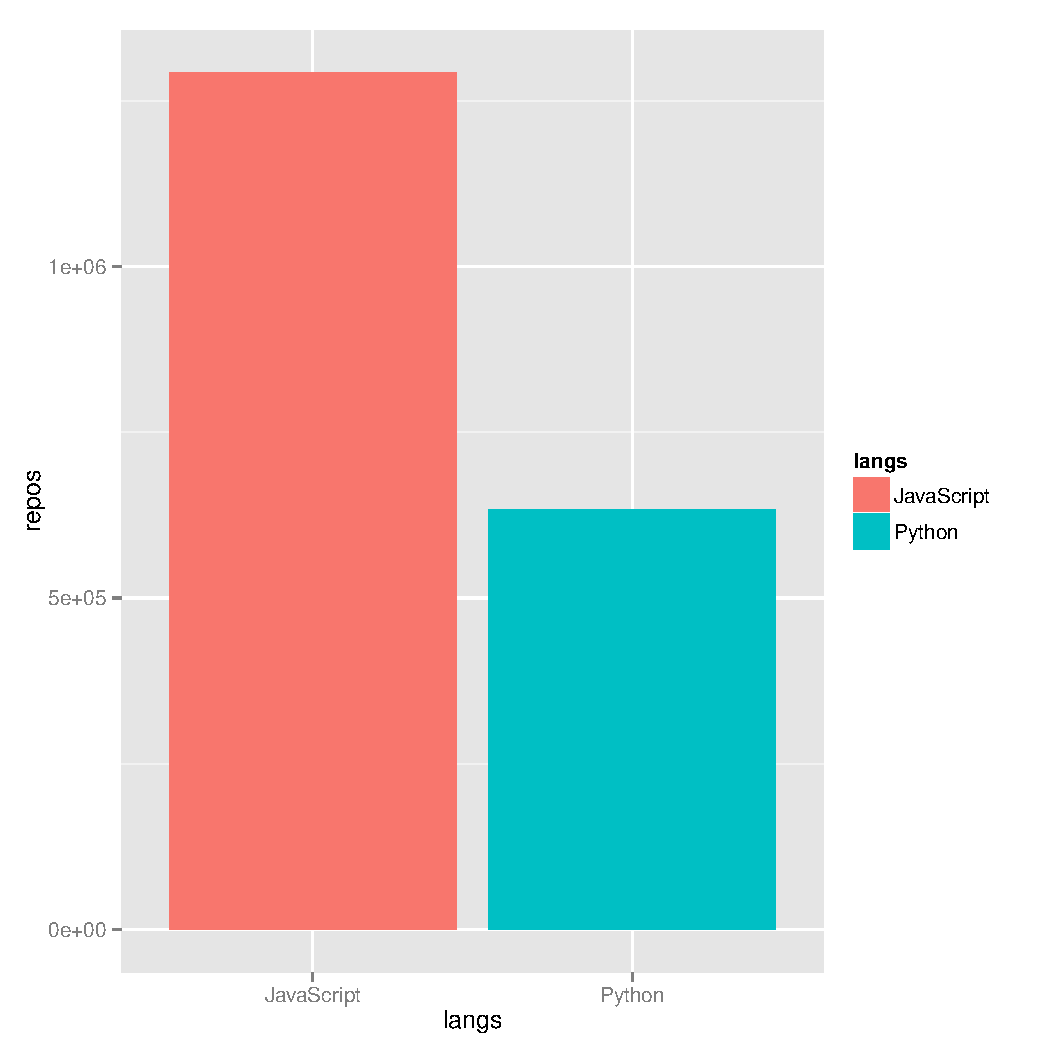
\includegraphics[width=\maxwidth]{figure/bar-1} \end{Schunk}
The graph below is a line diagram and I used powerful \textbf{ggplot} library to draw it. In the graph below, x-axis represents languages ie., JavaScript and Python, y-axis represents number of repositories.  

\begin{Schunk}
\begin{Sinput}
# Line chart
ggplot(data = df, aes(x = langs, y = repos, group = 1)) + geom_line(colour = "coral1", 
    size = 1) + geom_point(size = 3, fill = "white") + expand_limits(y = 0) + 
    scale_shape_manual(values = c(22, 21))
\end{Sinput}

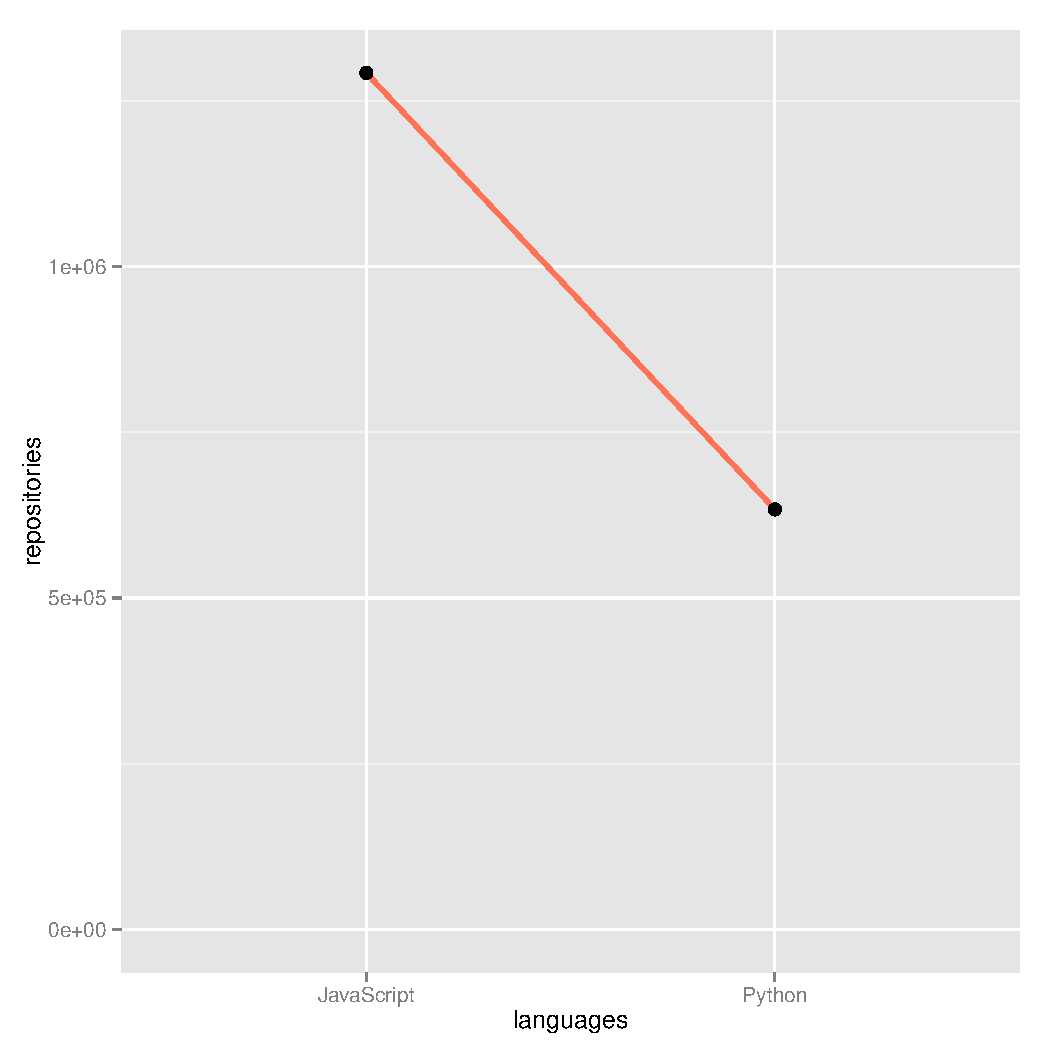
\includegraphics[width=\maxwidth]{figure/line-1} \begin{Sinput}
# end example code snip
\end{Sinput}
\end{Schunk}

\end{document}
